\documentclass{ceurart}
% Full-paper version of the manuscript; see README.md for build and review status.
% No class, page-geometry or body-font overrides are applied to the CEURART build.
\usepackage{listings}
\usepackage{tabularx}
\usepackage{booktabs}
\usepackage{tikz}
\usetikzlibrary{arrows.meta,positioning}
\usepackage{xurl}
\newcommand{\term}[1]{\texttt{#1}}
\lstset{basicstyle=\small\ttfamily,breaklines=true,columns=fullflexible,
  keepspaces=true,showstringspaces=false,frame=single,
  aboveskip=6pt,belowskip=6pt}
\emergencystretch=1em
\begin{document}

\copyrightyear{2027}
\copyrightclause{Copyright for this paper by its authors.
  Use permitted under Creative Commons License Attribution 4.0
  International (CC BY 4.0).}
\conference{SWAT4HCLS 2027, February 1--4, 2027, Basel, Switzerland}

\title{VCF Core: A Semantic Foundation for RDF Representations of VCF}

\author[1,2]{Elias Crum}[
orcid=0009-0005-3991-754X,
email=elias.crum@ugent.be
]
\cormark[1]
\author[2]{Bart Buelens}[
orcid=0000-0001-7734-3747,
email=bart.buelens@vito.be
]
\author[2]{Gökhan Ertaylan}[
orcid=0000-0001-5602-6435,
email=gokhan.ertaylan@vito.be
]
\author[1]{Ruben Taelman}[
orcid=0000-0001-5118-256X,
email=ruben.taelman@ugent.be
]
\address[1]{IDLab, Department of Electronics and Information Systems, Ghent University -- imec, Belgium}
\address[2]{Flemish institute for Technological Research (VITO) Mol, Belgium}
\cortext[1]{Corresponding author.}



% REVISED: abstract follows context, need, contribution, findings and prospects.
\begin{abstract}
Medical applications of genomic data depend on connecting variant observations to clinical information and biomedical knowledge. 
Linked Data offers a framework for this integration, but the Variant Call Format (VCF) does not natively provide an RDF representation of the observations and their interpretation context. 
We present VCF Core Vocabulary 2.1.2, a shared semantic target for representing VCF files, header declarations, records, annotations and sample data. The vocabulary integrates existing provenance and genomic models while retaining VCF-specific field definitions, ordering and missingness. 
Expanded sample calls expose individual values, whereas condensed, sample-ordered vectors provide an alternative for cohort data. 
Version-specific registries and validation profiles address VCF 4.1--4.5, including 122 reserved INFO and FORMAT declarations for VCF 4.5. 
A curated assessment records representation evidence for all 104 inventoried logical-model constructs and enforcement evidence for 87, and a set of 123 curated alignments documents connections to existing variation models and reference ontologies. 
We evaluate the vocabulary with executed checks rather than term counts. 
A specification-derived assessment of 94 requirements over VCF 4.1--4.5 supplies queries and expected answers authored in advance; replaying the 39 requirements that a ten-fixture subset exercises over graphs from a second, separately implemented producer gives agreement on 536 of 572 checks, 508 of them passing for both, with no divergence attributable to a representation gap. 
A semantic round-trip recovers the fixed columns and genotypes of all 35 records, in the expanded profile, from structured properties alone, and one integration example answers an allele-dependent question under VCF 4.5 local alleles with checked answers and recovered provenance. 
The replay also found a silent correctness defect in local-allele handling that per-producer testing had not, which we report as evidence for keeping representational mechanism, implementation and correctness apart. 
We then discuss how this foundation could support reusable conversion engines, traceable links to biomedical resources, and SPARQL queries combining genomic observations with medically relevant information.
\end{abstract}
\begin{keywords}
Variant Call Format\sep RDF\sep Genomic data\sep Vocabulary\sep Data integration\sep SHACL
\end{keywords}
\maketitle

% REVISED: motivation before technical detail; no first-ever conversion claim.
\section{Introduction}

Genomic data are increasingly useful in medicine when integrated with other patient, public and proprietary information. 
A drug-response assessment, for example, depends on the relationship between a patient's genomic findings, a prescribed medication, and the knowledge used to interpret that relationship~\cite{lee2022cpic}.
The presence of a variant alone does not establish these connections. 
Semantic approaches provide a basis for making such connections explicit: HERO-Genomics addresses integration of genomic and biomedical information, while Semantic Beacons demonstrates federated queries over variant data and public knowledge graphs~\cite{cazzaro2025hero,bodrug2025semantic}. 
Maturing investigation of genomic--medical data integration motivates a reusable representation of the source observations on which interpretation depends.

The Variant Call Format (VCF) is widely used to exchange genomic variant data~\cite{danecek2011vcf}. 
It already supports database identifiers, reference information and extensible annotations, so its limitation is not that data linking is impossible. 
Rather, VCF does not natively expose these elements and their relationships in a Findable, Accessible, Interoperable and Reusable (FAIR) way. 
Moreover, a value in a VCF file often depends on a header declaration, an ordered allele list, or the structure of a sample column for its interpretation~\cite{vcf45}. 
Converting only selected variant attributes can leave those dependencies implicit.
Linked Data and the Resource Description Framework (RDF) are therefore an attractive way to capture the full context of the information a VCF file carries.

Existing VCF-to-RDF approaches provide important foundations. 
The Genomic Feature and Variation Ontology (GFVO) includes VCF term coverage within a broader model of genomic features and variation, and VCF2RDF presents an isomorphic semantic mapping of the VCF format~\cite{baran2015gfvo,penha2017vcf2rdf}. 
The next step is therefore not to establish that VCF can be represented in RDF. 
It is to provide a shared, version-aware target that combines broad coverage of the source format with explicit connections to these existing models. 
Such a target would allow conversion and querying approaches to develop without each introducing its own interpretation of VCF structure.

Here, we present the VCF Core Vocabulary (\textit{vcfcv}) 2.1.2~\cite{vcfc210}, developed from our earlier VCF-RDFizer Vocabulary~\cite{crum2025semantifying}. 
The contribution combines source-context preservation, alternative sample representations, documented alignment, and coverage evidence across VCF 4.1--4.5. 
After introducing VCF and the model, we explain its relationship to existing work, assess its scope, and discuss how it could support integrated, medically relevant genomic querying. 
Throughout, \term{vcfc:} denotes \url{https://w3id.org/vcf-core/vocab#}.

% VCF introduction for readers who already understand RDF and vocabularies.
\section{VCF as a semantic representation problem}
\label{sec:vcf}

\subsection{What a VCF file describes}

A VCF file contains meta-information lines, a column-header line and data records. 
Meta-information lines beginning with \term{\#\#} identify the format version and can describe the reference sequence, genomic sequence segments called contigs, and the fields used in the records. 
The column header begins with \term{\#CHROM}. 
Each subsequent record describes a genomic position, the reference sequence at that position and one or more alternatives, together with observations and annotations~\cite{vcf45}. 
Table~\ref{tab:vcf} summarizes the main components.

\begin{table}[htbp]
\caption{VCF components and the interpretation context that an RDF representation needs to retain. INFO describes a record; FORMAT describes the contents of sample columns.}
\label{tab:vcf}
\centering\small
\begin{tabularx}{\linewidth}{@{}p{0.23\linewidth}X@{}}
\toprule
Component & Role in the source file \\
\midrule
Header declarations & Define field identifiers, types, cardinalities and descriptions, together with reference and processing context. \\
CHROM, POS, ID & Identify the reference contig, position and optional record identifiers. Position alone is not a globally unique variant identifier. \\
REF, ALT & Give the reference allele and ordered alternative alleles. An allele is a sequence alternative at the represented locus. \\
QUAL, FILTER, INFO & Describe call quality, filter status and record-level annotations, including producer-defined fields. \\
FORMAT and samples & Declare an ordered set of keys and give corresponding values for each sample, such as genotype (GT) and read depth (DP). \\
\bottomrule
\end{tabularx}
\end{table}

For example, a synthetic record at position 100 on contig 1 with reference allele A, alternative allele G and \term{FORMAT=GT:DP} may carry the sample values \term{0/1:42}, \term{0/0:18} and \term{./.:.} --- a heterozygous call at depth 42, a homozygous reference call at depth 18, and a sample whose genotype and depth are both missing. 
The slash separates unphased allele calls, while a vertical bar marks phased calls in which allele ordering is meaningful~\cite{vcf45}.

These compact encodings illustrate why representing VCF requires more than assigning predicates to columns. 
Genotype indices refer to the record's ordered allele list, and the meaning of a sample value depends on its FORMAT key. 
Likewise, a header's \term{Number=A} means one value per alternative allele, whereas \term{Number=R} includes the reference allele and \term{Number=G} depends on possible genotypes. 
The same key, such as DP, can occur in INFO and FORMAT without identifying the same observation~\cite{vcf45}.

\subsection{Why version and source context matter}

VCF 4.1--4.5 share these basic structures but differ in supported declarations and constraints~\cite{htsspecs,vcf45}. 
For example, CIPOS describes uncertainty around a reported position. 
Its declared cardinality changes from two values in VCF 4.1--4.3 to two per alternative allele in 4.4--4.5. 
VCF 4.5 also introduces local-allele cardinalities and base-modification fields. 
A common RDF model should support these developments without interpreting an older file under rules introduced later.

A source observation must also remain distinguishable from its biological interpretation. 
Two files may describe the same alteration with different quality scores or annotations. 
A sample column may represent a patient specimen, a pooled sample or a synthetic example. 
Neither records nor sample columns should therefore automatically be equated with normalized variants or patients.

\section{The VCF Core vocabulary}
\label{sec:design}

\subsection{Retaining observations and their provenance}

VCF Core separates a \term{VCFFile}, its \term{VCFHeader}, individual \term{VCFRecord} resources and a \term{VariantCall} associated with each record. 
The call groups quality, filter, annotation and genotype information; it is a modeling abstraction rather than an additional line in the source file. 
Figure~\ref{fig:model} shows this shared structure and the two sample representations.

The file specializes \term{dcat:Distribution} and \term{prov:Entity}, while records and calls provide further attachment points for provenance~\cite{prov2013,vcfc210}. 
File-based IRI templates preserve the relationship between source, record and field. 
Because a VCF identifier can be missing or non-unique, a producer must use a record identifier that distinguishes rows within the source. 
This approach allows observations from different files to remain separate even after they have been linked to a common biological entity.

The property \term{asSequenceAlteration} connects a record or call to a separately described Sequence Ontology (SO) sequence alteration~\cite{eilbeck2005so}. 
FALDO supplies location, reference and position descriptions, including uncertain positions where appropriate~\cite{bolleman2016faldo}. 
Thus, VCF Core does not introduce a competing general-purpose location model. 
Establishing cross-file links still requires compatible reference sequences and correct allele interpretation; the vocabulary provides the connection points rather than a normalization algorithm.

\begin{figure}[htbp]
\centering
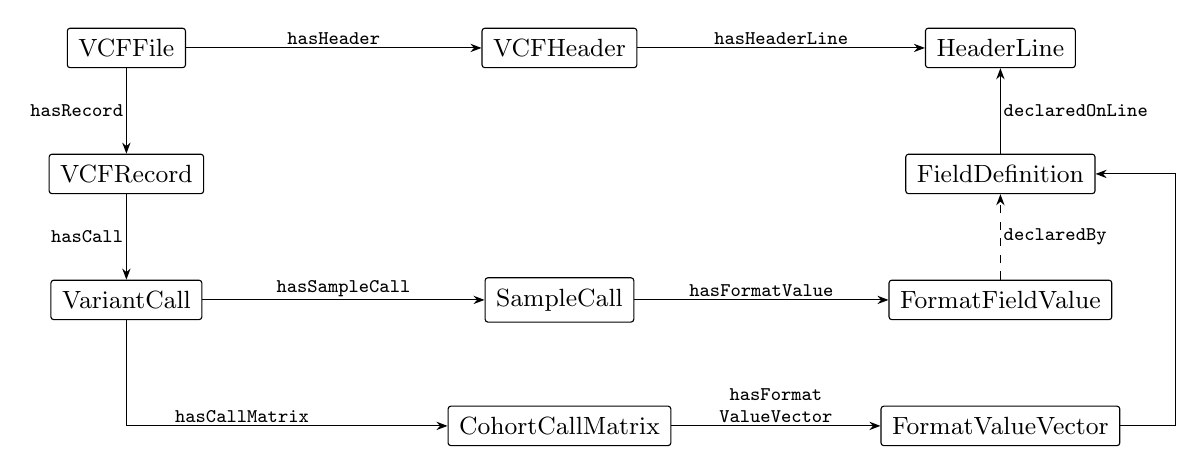
\begin{tikzpicture}[x=1mm,y=1mm,
  box/.style={draw,rounded corners=1pt,align=center,font=\small,inner sep=4pt},
  edge/.style={-{Stealth[length=4pt]},thin},
  lab/.style={font=\scriptsize\ttfamily,fill=white,inner sep=1pt,align=center}]
\node[box] (file) at (17,0) {VCFFile};
\node[box] (header) at (72,0) {VCFHeader};
\node[box] (line) at (128,0) {HeaderLine};
\node[box] (record) at (17,-16) {VCFRecord};
\node[box] (call) at (17,-32) {VariantCall};
\node[box] (definition) at (128,-16) {FieldDefinition};
\node[box] (sample) at (72,-32) {SampleCall};
\node[box] (value) at (128,-32) {FormatFieldValue};
\node[box] (matrix) at (72,-48) {CohortCallMatrix};
\node[box] (vector) at (128,-48) {FormatValueVector};
\draw[edge] (file) -- node[lab,above] {hasHeader} (header);
\draw[edge] (header) -- node[lab,above] {hasHeaderLine} (line);
\draw[edge] (file) -- node[lab,left] {hasRecord} (record);
\draw[edge] (record) -- node[lab,left] {hasCall} (call);
\draw[edge] (definition) -- node[lab,right] {declaredOnLine} (line);
\draw[edge] (call) -- node[lab,above] {hasSampleCall} (sample);
\draw[edge] (sample) -- node[lab,above] {hasFormatValue} (value);
\draw[edge] (call.south) |- node[lab,above,pos=0.68] {hasCallMatrix} (matrix);
\draw[edge] (matrix) -- node[lab,above] {hasFormat\\ValueVector} (vector);
\draw[edge,dashed] (value) -- node[lab,right] {declaredBy} (definition);
\draw[edge] (vector.east) -- ++(7,0) |- (definition.east);
\end{tikzpicture}
\caption{Selected VCF Core relationships; prefixes are omitted. Both sample profiles retain the file, record and header context. 
An expanded value can link to its definition through \term{declaredBy}; the equivalent relation is required for a condensed vector. 
Sample identity and ordering are described separately through \term{VCFSample} and \term{SampleSet}.}
\label{fig:model}
\end{figure}

\subsection{Making field interpretation explicit}


Header declarations are represented because they determine how values should be read: VCF Core gives each meta-information line type its own class and exposes a field definition's identifier, Number, Type, Description and optional source and version as data, with generic \term{HeaderAttribute} resources retaining producer-defined additions~\cite{vcfc210}.

Two modelling decisions in this area carry most of the weight. 
First, a standardized definition and its occurrence in a file are kept apart --- the reserved FORMAT/DP definition describes a key the specification supplies, while a header line records what one file declares --- so \term{FieldDefinition} and \term{HeaderLine} are distinct resources joined by \term{declaredOnLine}, and values reach their declaration through \term{declaredBy}. 
Without that separation a registry entry would be forged into every file that never declared it. 
Second, lexical and parsed forms are both retained: \term{fieldValue} keeps the source token or list while optional integer, decimal and boolean properties serve scalar queries, so a missing depth is never coerced to zero and a non-finite float is never forced into \term{xsd:decimal}. 
Standalone missing values use \term{vcfc:Null}, and ordered allele resources index REF at zero and ALT upwards, which is what makes a genotype integer and an allele-dependent annotation resolvable. 
Raw source text may be retained alongside, but a preserved string is never counted as structured coverage.

\subsection{Choosing how sample data are represented}
\label{sec:profiles}

The expanded profile connects each call to per-sample \term{SampleCall} resources and individual \term{FormatFieldValue} resources. 
This makes values directly accessible through graph patterns and allows an application to annotate a particular sample observation. 
A \term{VCFSample} identifies the source column; linking it to a biological specimen or patient is a separate integration task. 
Expanded representation is applicable to both single- and multi-sample files when direct access justifies the additional graph structure.

Condensed representation associates each call with a cohort matrix. 
The \term{CohortCallMatrix} groups one \term{FormatValueVector} for each represented FORMAT key. 
A shared \term{SampleSet} identifies samples by name and one-based index. 
Each vector specifies its definition, encoding and payload. 
The initial \term{VCFTextVector} encoding stores tab-separated sample values in index order, including missing values. 
The synthetic example therefore produces GT values \term{0/1}, \term{0/0}, \term{./.} and DP values \term{42}, \term{18}, \term{.} in corresponding positions.
% TODO: cite the GeoSparql encoding paper ruben suggested in here as grounding to this apporach

This is a change in graph granularity, not a replacement of sample observations by cohort summaries. 
Individual condensed cells require decoding before per-sample comparisons; they are not directly bound by ordinary basic graph patterns. 
For $R$ records, $S$ samples and $F$ FORMAT keys, expanded materialization creates $RS$ sample calls and $RSF$ value resources. 
Condensed materialization creates $S$ sample resources, one sample set, $R$ matrices and $RF$ vectors. 
These counts exclude shared metadata and do not establish savings in bytes, memory or query time. 
The underlying payload still contains $RSF$ values.

Listing~\ref{lst:depth} illustrates direct expanded access. 
On the supplied synthetic graph it returns SAMPLE1 with depth 42; decoding the condensed graph gives the same selection and recovers the same six FORMAT cells. 
The threshold is illustrative, not a clinical quality standard. 
This bounded example establishes neither general conversion fidelity nor clinical validity.

\begin{lstlisting}[float=htbp,caption={An expanded-profile query over the supplied synthetic example.},label={lst:depth}]
PREFIX vcfc: <https://w3id.org/vcf-core/vocab#>
SELECT ?sampleName ?depth WHERE {
  ?file vcfc:representationProfile vcfc:ExpandedRepresentation ;
        vcfc:hasRecord/vcfc:hasCall/vcfc:hasSampleCall ?call .
  ?call vcfc:forSample/vcfc:sampleName ?sampleName ;
        vcfc:hasFormatValue ?value .
  ?value vcfc:declaredBy/vcfc:fieldId "DP" ;
         vcfc:fieldValueInteger ?depth .
  FILTER (?depth >= 20)
}
\end{lstlisting}

% REVISED: prior work is a foundation, not an unsupported coverage leaderboard.
\section{Building on existing semantic models}
\label{sec:alignments}

\subsection{Complementary contributions}

The usefulness of VCF Core depends on its relationship to the models already used for genomic data. 
GFVO was developed from several genomic formats, explicitly including VCF 4.1 and 4.2~\cite{baran2015gfvo}. 
VCF2RDF demonstrated source-preserving semantic conversion~\cite{penha2017vcf2rdf}. 
HERO-Genomics includes VCF files and records within a broader integration model, while the Genome Variation Ontology (GVO) addresses detailed variation descriptions, including complex structural variants~\cite{cazzaro2025hero,kawashima2023gvo}. 
The GA4GH Variation Representation Specification (VRS) provides computable variation descriptions and federated identification, rather than a representation of every source-file detail~\cite{wagner2021vrs}. 
These are complementary purposes, not successive attempts at the same task.

To place VCF Core among them without asserting superiority, we inspected the published artifact of each model and scored nine retrieval criteria drawn from the interpretation context a VCF file carries about itself (Table~\ref{tab:comparison}). 
Each criterion is a question about what can be retrieved, not a judgement of quality, and each verdict names the term or absence it rests on. 
GA4GH VRS is deliberately not scored: it describes computable variation identity rather than a source file, so scoring it against file-format criteria would manufacture a contrast its authors never sought.

\begin{table}[htbp]
\caption{What each inspected artifact lets a consumer retrieve. \textbf{E}~explicitly represented; \textbf{C}~representable with additional conventions; \textbf{S}~outside the model's stated scope, which is not a defect. Scored against GFVO (BioInterchange \texttt{master}), HERO-Genomics 1.0, GVO (\texttt{versionInfo} 2021-11-18) and the VCF2RDF term set (\texttt{v4\_2}), GFVO and HERO-Genomics retrieved 2026-09-12, GVO and the VCF2RDF term set 2026-09-13.}
\label{tab:comparison}
\centering\small
\begin{tabularx}{\linewidth}{@{}Xccccc@{}}
\toprule
Retrieval criterion & \rotatebox{90}{VCF Core} & \rotatebox{90}{GFVO} & \rotatebox{90}{HERO} & \rotatebox{90}{GVO} & \rotatebox{90}{VCF2RDF} \\
\midrule
A record traces to its source file & E & E & E & S & C \\
A declaration exposes ID, Number, Type & E & S & S & S & E \\
The file's VCF version is readable & E & S & S & S & C \\
ALT allele \emph{n} is addressable by index & E & C & C & S & C \\
Ploidy, calls and phasing are separable & E & C & C & S & C \\
A (sample, field) value without splitting a cell & E & C & C & S & C \\
A \texttt{Number=A/R/G} item binds to its allele & E & C & C & S & C \\
An explicit \texttt{.} differs from ``not stated'' & E & S & C & C & C \\
The sample encoding is readable from the graph & E & S & S & S & S \\
\bottomrule
\end{tabularx}
\end{table}

Two contrasts explain the pattern. 
HERO-Genomics and GVO both retain the INFO column as a single literal --- our alignment set records \term{hero:vcfInfo} and \term{gvo:info} as exact matches to \term{vcfc:infoRaw} --- so every INFO-derived question requires re-parsing that string and supplying the cardinality rule from outside the graph. 
GFVO makes the opposite choice, modelling particular field \emph{meanings} as first-class concepts (\term{AlleleCount}, \term{Coverage}, \term{MappingQuality}), which answers those fields well and leaves the declaration mechanism unaddressed. 
VCF2RDF is the instructive case: its published term set does define \term{Number}, \term{Type} and \term{Description} as dereferenceable terms, so the cardinality rule is named rather than left outside the vocabulary --- but with no allele-index term a consumer must still split the list and count ALT alleles by re-reading a literal. 
Having the declaration is necessary and, alone, insufficient; binding a value to an allele is the part that must be represented rather than inferred.

These verdicts are bounded in three ways. 
The criteria were chosen for the interpretation problem VCF Core addresses, so this is not a neutral ranking --- a matrix chosen by GVO's authors would look different and would be equally legitimate. 
GVO's column is S in every row but missingness, because the retrieved ontology declares 48 classes, 12 datatype properties and \emph{no} object properties: a model of variation types, doing something other than file modelling. 
Missingness scores C there only because a literal-valued property can carry a dot, while distinguishing that from an absent triple remains a convention the ontology does not supply. 
The VCF2RDF column rests on a published term set carrying specification glosses rather than RDF axioms, and on no converter output, so what its graphs contain is still taken from its paper. 
Finally, ``requires additional conventions'' states what an inspected artifact establishes, never that a model's community could not represent something.

\subsection{Reuse and curated alignment}

Direct reuse and cross-model alignment are kept distinct. 
PROV, DCAT, SO and FALDO terms contribute to the core representation through axioms or instance descriptions. 
The accompanying alignment set documents correspondences to models whose assumptions do not always coincide with a source-oriented VCF representation. 
Table~\ref{tab:alignments} summarizes the 123 mappings from 65 VCF Core terms to 103 external terms~\cite{vcfc210}.

\begin{table}[htbp]
\caption{Curated alignment targets. Counts describe the mapping set, not comparative specification coverage or demonstrated instance-level interoperability.}
\label{tab:alignments}
\centering\small
\begin{tabularx}{\linewidth}{@{}p{0.24\linewidth}rX@{}}
\toprule
Target & Mappings & Connection to VCF Core \\
\midrule
GVO & 39 & Variation and VCF-related properties. \\
HERO-Genomics & 17 & File, record and observation descriptions. \\
GA4GH VRS 2.0 & 15 & Computable descriptions of variation. \\
GFVO & 14 & Genomic features and field-related concepts. \\
Med2RDF & 3 & VCF-oriented allele properties. \\
SO, ChEBI, GENO, FALDO & 35 & Alteration types, modifications, genotype concepts and locations. \\
\bottomrule
\end{tabularx}
\end{table}

Mappings are curated in the Simple Standard for Sharing Ontological Mappings (SSSOM), which records the mapping predicate, justification and associated metadata~\cite{matentzoglu2022sssom}. 
A generated Turtle bridge provides the RDF form. 
Of the 123 mappings, 48 are also asserted inline in ontology modules; the remaining 75 are available through the separately loaded bridge. 
Keeping this distinction visible lets consumers identify which mapping assertions accompany the core and which require an additional module.
% TODO: Add link to specific locaiton in git repo here

The set contains 57 \term{skos:exactMatch}, 40 \term{skos:closeMatch}, 16 \term{skos:relatedMatch} and 10 \term{skos:narrowMatch} assertions. 
These do not establish OWL class or property equivalence, nor do they generate the instance links needed for a biomedical query. 
They nevertheless have defined semantics: \term{skos:exactMatch} is transitive, whereas \term{skos:closeMatch} is not~\cite{skos2009}. 
Consequently, mixed mapping paths cannot be treated as unrestricted rules for predicate substitution, and mappings between different VRS releases require explicit review.

% TODO: refine this section
The repository additionally preserves 116 SSSOM mappings from work in the 2025 SWAT4HCLS BioHackathon separately from VCF Core's own assertions~\cite{bh25}. 
Of 47 terms previously recorded as lacking a VRS counterpart, eight have a source-oriented VCF Core counterpart, including file, quality, and as-written allele concepts. 
This illustrates the contribution of retaining source semantics alongside biological models; it does not mean that the 39 remaining annotation and interpretation concepts should all become VCF Core terms.

\section{Specification coverage and implementation evidence}
\label{sec:coverage}

\subsection{One representation with version-specific rules}

VCF Core uses one shared model for common structures and version-specific registries and validation overlays for VCF 4.1--4.5~\cite{vcfc210}. 
The registries contain 40, 40, 67, 78 and 122 explicit reserved declarations, respectively. 
For VCF 4.5 these comprise 51 INFO and 71 FORMAT definitions, including three entries for parameterized base-modification key families. 
Prose-only fields in older versions are not assigned Number or Type constraints absent from their specifications.

The overlays condition rules on the owning file's declared version. 
Thus, the CIPOS example in Section~\ref{sec:vcf} can be assessed under the appropriate historical or current rule, while the LA, LR, LG and M cardinalities are restricted to VCF 4.5. 
Shared validation is divided into portable SHACL structure checks, SPARQL-based cross-resource checks and raw/parsed-value consistency checks~\cite{shacl2017,vcfc210}. 
This organization permits different validator capabilities without implying that each layer independently validates the entire format.

\subsection{What the evidence establishes, and at what strength}
\label{sec:evidence}

Coverage claims are easy to overstate because three different things are routinely reported as one number. 
We keep them apart. 
\emph{A mechanism exists} when a term, rule or documented pattern is available; this establishes nothing about correct instantiation. 
\emph{An example instantiates it} when a fixture demonstrates the mechanism in use; this establishes nothing about general correctness. 
\emph{Behaviour is independently checked} when an executed query agrees with an expected answer established separately from the code that produced the graph. 
Only the third supports a correctness claim, and only within what was tested.

Two assessments and two cross-checks address three questions: whether VCF Core preserves the intended meaning of the constructs it claims to support (RQ1); whether the version-specific artifacts and the two sample profiles behave as documented (RQ2); and whether the result supports a reproducible integration task that retains source context (RQ3).

\paragraph{Mechanism.}
The curated VCF 4.5 inventory enumerates 104 logical constructs across file and header organization, declarations, types and cardinalities, lexical rules, fixed fields and alleles, genotypes, structural variation, repeats and gVCF. 
All 104 have preserved, structured representations and 87 additionally have an enforcement rule. 
Separately, all 333 reserved Number/Type rows extracted from the specification texts match the versioned registries~\cite{vcfc210}. 
Those 333 rows --- 31, 31, 69, 79 and 123 per version --- are the keys each source declares explicitly in \texttt{\#\#INFO=}/\texttt{\#\#FORMAT=} blocks or reserved-key tables, and are a different population from the registry entries counted above. 
VCF 4.1 and 4.2 each define a further 29 reserved keys in prose bullets that give no Number and, for INFO, no Type; those rows are inventoried but cannot be compared, so this agreement figure is weighted towards VCF 4.3--4.5. 
The inventory was curated by the vocabulary's developers, so it maps what its authors listed and cannot reveal an omission nobody listed.

\paragraph{Instantiation and independent checking.}
The specification-derived assessment reads information requirements from pinned VCF 4.1--4.5 sources and tests them against fixtures. 
It comprises 94 requirements over 210 cases; each case pairs a SPARQL query with an expected answer authored from the specification text \emph{before} the query was run, and every passing query is re-run against an emptied graph as a negative probe. 
Executing every case on both sample profiles yields 840 nominal query runs, but 165 cases score the identical query and expected answer on two axes, so the independent figure is \textbf{465 distinct executions}. 
Coverage is reported per version because requirements apply per version, and an untested requirement scores zero rather than being excluded (Table~\ref{tab:evidence}).

\begin{table}[htbp]
\caption{Reported evidence, its denominator and the claim it supports. The denominators count different things and must not be combined into a single percentage.}
\label{tab:evidence}
\centering\small
\begin{tabularx}{\linewidth}{@{}p{0.28\linewidth}p{0.15\linewidth}X@{}}
\toprule
Assessment & Result & Supported interpretation \\
\midrule
Curated VCF 4.5 inventory & 104/104 & All inventoried logical constructs have preserved, structured representations. \\
Enforcement within that inventory & 87/104 & A stated requirement is checked for these constructs. \\
Reserved Number/Type rows & 333/333 & Extracted declarations match the version-specific artifacts. \\
Requirements with a passing test, by version & 32/69, 34/72, 35/74, 38/83, 51/91 & Conservative demonstrated coverage for VCF 4.1--4.5; untested requirements score zero. \\
Distinct executed checks & 465 & Query runs that are not a repeat of an identical check. \\
Cross-producer replay & 508/572 & Checks on which the vocabulary's materializer and the cited converter agree and both pass. \\
Semantic round-trip & 35/35 records & Fixed columns and genotypes recovered from structured properties alone. \\
Recorded full validation run & 21 fixtures & These examples pass the implemented validation layers. \\
\bottomrule
\end{tabularx}
\end{table}

A previous version of this assessment reported 491 reviewed requirements of which 133 had complete evidence. 
That generation has been superseded: requirements are now scored per version and per profile, and no single figure corresponds to the earlier 133.

\subsection{Whether the claimed coverage survives a second producer}
\label{sec:crossproducer}

The assessment above builds its witness graphs with the vocabulary repository's own materializer, whereas the implementation this paper cites is a separate program, and nothing had established that a query and expected answer written against one also holds over the other --- the gap between ``the vocabulary can express this'' and ``the software people will use does''. 
The two programs share an author but no code: one materializes graphs from a Python fixture builder, the other from RML mappings and streaming emitters. 
Independence here therefore means independent implementations, not independent authorship, and the check is correspondingly weaker than third-party reproduction.

We replayed the existing queries, against the existing reviewed expected answers, over graphs produced by VCF-RDFizer: ten fixtures spanning VCF 4.1--4.5 and the difficult decisions above, each converted in both profiles, giving 572 checks over 143 cases and 39 requirements. 
The producers agree on 536 checks and both pass on 508; 34 requirements agree on every check and 28 of those pass throughout. 
Every check they agree on by both failing is a condensed-profile structure query, the documented storage trade-off.

The exercise earned its keep by failing. 
Its first run diverged on 15 requirements, nine of which were converter defects precise enough to fix. 
One was a silent correctness defect in VCF 4.5 local alleles, this paper's own headline feature: \term{Number=LA} and \term{Number=LR} items were bound to allele indices positionally, ignoring the sample's \texttt{LAA} subset, so a depth list of \texttt{20,30,10} under \texttt{LAA=2,4} landed on alleles 0, 1 and 2 instead of 0, 2 and 4 --- plausible, well-formed values on the wrong alleles, which no existing test caught because every existing test ran against the other producer. 
Five requirements still diverge: a QUAL datatype the vocabulary deliberately leaves open, three structured accessors the converter has not built (one of them the condensed-vector decoding path), and one empty-list encoding convention. 
None is a case of the vocabulary being unable to express something --- across all 572 checks, zero divergences trace to a representation gap.

A complementary check recovers logical content rather than comparing query answers. 
Across the same ten fixtures we reconstruct CHROM, POS, ID, REF, ALT, QUAL, FILTER and the GT subfield from the RDF alone: REF and ALT from ordered \term{alleleIndex}/\term{alleleValue} resources, GT from ordered \term{GenotypeAlleleCall} resources with their phasing status, so no untouched source string serves as a shortcut. 
All 35 records are recovered, with three bounds, all by design: INFO and the non-GT FORMAT subfields are out of scope; the check runs on expanded-profile graphs only, since decoding a condensed vector needs the accessor requirement R21 identifies as missing; and in the local-allele fixture, where each site is written once locally and once globally, matching on position confirms one recovery per site rather than both. 
It is not whole-file reconstruction.

\paragraph{Where the two sample profiles agree.}
Because every case runs in both profiles, the profile claim can be stated precisely rather than asserted. 
The profiles return the same outcome on 252 of 286 comparable checks, and the 34 disagreements fall on nine requirements, every one reading a FORMAT-scoped value: genotype structure, trailing-field missingness, sample-local allele and base-modification items, and repeat components. 
Record-level file, header, declaration and allele questions agree on every check in both profiles. 
The supported claim is therefore that the profiles are equivalent for file, header, record and record-level allele questions and divergent by design wherever a query walks per-sample resources. 
Two of the nine are local-allele requirements, so this paper's headline feature is among those a condensed graph answers less completely.

\paragraph{Answers to the three questions.}
RQ1 is answered for the 53 of 94 requirements with at least one executed case, the great majority passing. 
RQ2 is answered for 17 of the 36 version-conditioned requirements, with the profiles behaving as documented: equivalent above the sample level, divergent below it. 
RQ3 is answered for 27 of the 38 requirements on the provenance chain an integration query must traverse, which Section~\ref{sec:integration} then exercises end to end. 
None of these fractions is a conformance claim; each is the share of requirements whose behaviour has been checked at all.

\paragraph{Remaining gaps, classified.}
Of the requirements exercised, none reveals a representation gap. 
One correctness defect was found and fixed; three requirements await structured accessors in the converter; one reflects an interpretation the vocabulary deliberately permits both ways; one is an encoding convention. 
The largest limitation is absence of evidence rather than negative evidence: 41 of the 94 requirements have no test case yet, concentrated in structural-variant fields with version-specific semantics. 
Allele-dependent values, this paper's central modelling claim, are tested for 4 of the 11 requirements that bear on them --- adequate to demonstrate the mechanism and to catch the defect above, not adequate to claim general correctness. 
Outside that classification, four validator findings remain from the release's own conformance checks: custom structured-header IDs can be absent or duplicated without rejection; numeric base-modification keys can be accepted with incorrect Number/Type pairs; a partially missing phase-set-list example is rejected under an unresolved interpretation; and mixed LF/CRLF line endings are rejected under an unconfirmed reading of the specification. 
Byte-level checking is reported separately, and neither BCF binary layout nor byte-for-byte reconstruction is a target of the logical model.

\subsection{Implementation and reproducibility}
\label{sec:implementation}

The release provides OWL/Turtle modules, SHACL profiles, examples, versioned registries, SSSOM mappings and documentation~\cite{vcfc210}. 
VCF-RDFizer supplies a separate implementation: release 3.0.3 constructs file and record context with RML mappings and produces expanded or condensed sample structures through streaming emitters~\cite{vcfrConverter2026}. 
The Section~\ref{sec:evidence} assessment was produced with VCF Core 2.1.2 and the vocabulary's own materializer, with no converter involvement; all converter-dependent results (Sections~\ref{sec:crossproducer}--\ref{sec:integration}) used VCF-RDFizer 3.0.3, the release that carries the corrections the cross-producer check prompted. 
Both are tagged, so every figure below comes from a released artifact rather than a working branch. 
Converting the Section~\ref{sec:profiles} example emits 242 expanded and 168 condensed triples, drawing on 93 and 80 distinct VCF Core terms respectively. 
Every one of those terms is declared in VCF Core 2.1.2, and both graphs conform, with no violations, to the shared and the VCF 4.5 SHACL profile when the shapes are loaded with the vocabulary and RDFS inference, as the vocabulary's own validation does. 
The depth query in Listing~\ref{lst:depth} returns its expected single row against the expanded graph. 
The converter pins no vocabulary version, so this relationship is established by the behaviour recorded here rather than by a declaration, and it is evidence for the terms these graphs exercise, not for all 467 declared terms or for every historical VCF version.

Two pinning limitations are worth stating plainly because they affect reproduction. 
The published container image lags the source release: version-tagged images exist, but the newest is 3.0.2, which predates the corrections, so reproducing the results above requires building the image from the 3.0.3 source rather than pulling it. The toolchain inside that image is also not independently pinned. 
The counts above are converter output; the hand-authored illustration file in the release is smaller, because it omits the allele resources and per-sample genotype and allele-call resources that the converter materializes.

The recorded validation run accepts 21 fixtures and includes a negative control, alongside a regression suite of 101 tests. 
The published workflow recomputes the reported counts and checks evidence references against the maintained artifacts, and each result in Section~\ref{sec:evidence} has a script that reproduces it from the pinned inputs. 
Review of coverage judgements and mappings nonetheless remains a human task. 
The established result is full representation of the curated VCF 4.5 inventory with version-aware support across VCF 4.1--4.5, demonstrated to be reproducible with an independent converter on the subset tested --- not complete conformance.

\subsection{One integration example, with checked answers}
\label{sec:integration}

The claims above concern representation and query behaviour within the VCF world. 
To test whether the retained context survives contact with an external annotation, we ran one small end-to-end example and checked its answers against expectations authored in advance.

The example is bounded to a single difficulty: allele-dependent values under VCF 4.5 local alleles. 
\texttt{LAD} is declared \texttt{Number=LR}, meaning one value per allele of \emph{the sample's own} local allele subset named by \texttt{LAA}, not per entry of the record's ALT column. 
Answering ``how deep is this alteration in this sample?'' therefore requires the declaration, the sample's \texttt{LAA} and the allele's ordinal simultaneously. 
The input is a pinned four-site, single-sample VCF 4.5 fixture, each site written twice, once with local alleles and once globally; the annotations are a local, explicitly synthetic snapshot of five flagged alterations, labelled as such in the file, and local rather than federated so the example returns the same answer on every run. 
The link is made in the query rather than by pre-minted identifiers: an annotation names an alteration by contig, position, reference and alternate allele, and the query joins on those four literals. 
Three assumptions are recorded because they are what would break the link --- a shared assembly, as-written allele identity with no normalization or VRS matching, and that a VCF sample column is a sample and not a patient.

Asking which flagged alterations have supporting read depth of at least 20 returns two rows, identical to the expected answers: \texttt{chr1:1~G>C} at depth 30 and \texttt{chr1:2~A>T} at depth 25, each traced to its file, record, sample and the FORMAT declaration that gives the field its cardinality. 
The three flagged alterations absent from the answer are each absent for a stated reason rather than by oversight.

The example is worth reporting because of what it does under a wrong implementation. 
Run against converter output from before the local-allele correction, the same query and the same annotations return \emph{two rows again} --- but \texttt{chr1:1~G>A} at 30 and \texttt{chr1:2~A>C} at 25, the two alterations a positional reading of \texttt{Number=LR} would wrongly report, at exactly the depths predicted in advance. 
A check comparing result counts passes both graphs. 
This is the concrete form of the paper's argument: retaining the declaration, the local allele set and the allele ordinal is not bookkeeping, because dropping it yields a plausible, well-formed, wrong answer delivered with complete provenance.

What this example demonstrates is that the representation carries the interpretation context, that a mapping rule connects it to external annotation, and that the answers match those authored beforehand. 
What it does not demonstrate is equally clear: the input is synthetic and tiny, the annotations are invented and carry no biological or clinical meaning, the link assumes as-written allele identity, and a single fixture establishes correct local-allele handling here rather than in general.

% NEW: the following scenarios are prospective, not additional evaluation results.
\section{Discussion}
\label{sec:discussion}

\subsection{Connecting source observations to biomedical knowledge}

VCF Core can make more of the evidence already present in a VCF file available to semantic applications. It retains observations and their interpretation context, while other models describe specimens, patients, diseases, treatments and biological variation. These layers can develop independently when their relationships are explicit.

Two laboratories reporting the same alteration in separate files could, after reference-aware normalization, link to a common variation description while each retains its own quality values, sample identities and provenance --- so a disease association attaches to the description once rather than being copied into every source record, and a revised interpretation can be retrieved alongside the original observations. PROV, FALDO and the published alignments are starting points; the normalization and instance mappings themselves remain to be implemented and evaluated.

Sample identity needs the same separation. In a tumour/normal analysis two columns may be different specimens from one patient, and treating column names as patient identifiers destroys that distinction. An integration layer can link each \term{VCFSample} to its specimen and both specimens to the patient through a biomedical model such as HERO-Genomics~\cite{cazzaro2025hero}; VCF Core preserves the source side without replacing the clinical one.

\subsection{A shared target for conversion engines}

A reusable vocabulary also separates conversion strategy from representation decisions. A clinical site converting one sample for inspection and a research group converting a cohort can choose different sample profiles --- expanded values for direct annotation, condensed vectors with selective expansion for scale --- while retaining the same file, header and record model rather than growing incompatible vocabularies per workload. A pipeline spanning VCF 4.2 and 4.5 data can likewise select the registry and validation overlay from \term{fileFormat} instead of silently imposing the newest cardinality on an older declaration.

That suggests an evaluation order for future work: compare recovered source values and query answers first, as Section~\ref{sec:crossproducer} does, and only then measure conversion time, peak memory, serialized size and loading cost. Section~\ref{sec:profiles} is explicit that the profiles trade query granularity rather than demonstrated storage savings, and the present results do not establish which implementation is most efficient.

\subsection{SPARQL questions that combine genomic and clinical evidence}
\label{sec:clinicalqueries}

Section~\ref{sec:integration} established the pattern at the smallest scale that requires it: an external annotation joined to sample-level evidence, with the answer depending on interpretation context that the representation retains. 
The questions below extend that pattern to clinical settings. 
They are proposed research scenarios and \emph{not} evaluated workflows: unlike the example in Section~\ref{sec:integration}, none has been executed, and each requires additional biomedical data, reviewed instance mappings and appropriate access controls. 
SPARQL provides the query structure; it does not supply missing interpretation or establish that a returned result is clinically actionable.

\paragraph{Three questions.}
A \emph{pharmacogenomic} review asks which patients with an active clopidogrel prescription have an externally established CYP2C19 phenotype relevant to a guideline for their indication, and which source observations support that assessment; the CPIC guideline shows why phenotype and indication both matter~\cite{lee2022cpic}, and a workflow such as PharmCAT separates variant processing, allele matching and clinical interpretation~\cite{pharmcatmethods} --- steps that must not collapse into reading one genotype token as a metabolizer phenotype. 
A \emph{rare-disease} investigation asks which candidate alterations lie in genes associated with diseases sharing the patient's recorded phenotypic features, joining specimen-linked calls to normalized alterations, gene associations and phenotype descriptions such as HPO~\cite{hpo}; its governing constraint is that a row absent from a variant-only VCF is not evidence that a parent is homozygous reference. 
An \emph{oncology} review asks which alterations detected in a tumour have curated therapeutic evidence for the patient's cancer type, joining a resource such as CIViC~\cite{griffith2017civic} to normalized alterations and retrieving tumour and normal calls through their specimen links; a missing normal call likewise remains missing evidence, not proof of tumour specificity.

Each reaches its sample-level evidence through the same declaration-to-value path that Section~\ref{sec:integration} executes, and each needs clinical assertions from an application schema that is not part of VCF Core. 
The vocabulary retains the observations; completeness, segregation and therapeutic interpretation require evidence it does not carry.

These scenarios could be implemented over a materialized graph or, where source interfaces and authorization permit, through federated SPARQL as demonstrated in related work~\cite{bodrug2025semantic}. Availability of RDF and vocabulary alignments alone does not guarantee complete or performant answers. Future experiments should evaluate answer correctness, instance-link accuracy, provenance recovery and source availability before making claims about medical utility or query speed. The opportunity is to investigate these questions against a common representation instead of repeatedly reconstructing VCF semantics within each application.

\section{Conclusion}

VCF Core provides a shared semantic foundation for representing VCF observations together with the context needed to interpret them. 
It combines reuse of existing models, explicit source structure, alternative sample representations and version-specific artifacts for VCF 4.1--4.5. 
All 104 constructs in the curated VCF 4.5 inventory are represented, and the claims that matter have been executed rather than asserted: the specification-derived checks agree across a second producer on 536 of 572 replayed checks with no divergence traceable to the vocabulary, all 35 records round-trip through structured properties, and one integration example returns answers authored in advance together with their source provenance.

The remaining work is specific rather than general. 
Evidence is absent for 41 of the 94 requirements, concentrated in structural-variant fields, and thinner than we would like for allele-dependent values in particular; three structured accessors are not yet implemented in the cited converter; one QUAL datatype question is an interpretation the vocabulary deliberately leaves open; and the per-sample condensed profile cannot yet answer the hardest missingness question. 
None of these is a representation gap, and none is hypothetical --- each is a named requirement with a recorded result.

What this foundation makes practical is the step from representing genomic files to connecting their contents with biomedical knowledge. 
Conversion engines can target the same model, integration layers can preserve the distinction between observations and interpretations, and SPARQL studies can examine medically relevant questions with traceable source evidence. 
The clinical scenarios in Section~\ref{sec:clinicalqueries} remain future work: the VCF-side representation they would build on is in place and checked, while the biomedical models and reviewed instance mappings they equally require are not.

\begin{acknowledgments}
Project funding provided from the Research Foundation -- Flanders (FWO) (SB Fellowship 1S27825N).
Ruben Taelman is a postdoctoral fellow of the Research Foundation -- Flanders (FWO) (1202124N).
\end{acknowledgments}

\section*{Declaration on Generative AI}
OpenAI Codex and Claude assisted with preparatory work on the vocabulary, assessment artifacts and manuscript. ChatGPT assisted with restructuring, prose revision, reference checks and prospective query examples. 

\label{endofmain}

{\interlinepenalty=10000
\bibliography{sources}}
\end{document}
